\chapter{Explaining Algorithm Performance Distributions Through Interpretable Statistics}
\label{sec:ch09:dist_explain}


\section{Introduction}
\label{sec:ch09:intro}

Empirical performance models (\glspl{epm}) are data-driven predictive models that learn the relationship between problem instance features and an algorithm performance metric, such as expected running time or solution quality. They serve as critical components in automated algorithm selection, configuration, and parameter tuning across various domains, including compiler optimisation, database query optimisation, and machine learning.

While traditional \glspl{epm} predict a single expected value (typically mean running time), they fail to account for the stochastic nature of modern randomised algorithms. For combinatorial search and optimisation, state-of-the-art solvers rely heavily on randomisation to navigate vast search spaces, resulting in running times that vary substantially across runs on the same instance~\citep{HooStu04}. Consequently, capturing and explaining the full performance distribution—rather than just the mean—is essential for risk-sensitive applications where tail behaviour, failure rates, or consistency guarantees are critical.

To address this, recent approaches such as DistNet~\citep{EggEtAl18} model full per-instance running time distributions. However, these methods are either too compute-intensive or fail to provide explainable insights. Indeed, while \glspl{epm} have traditionally been used to analyse algorithm behaviour (see, e.g.,~\citealp{HutEtAl13}), existing explainability techniques are restricted to single-value predictors. This creates a fundamental discrepancy: the algorithms of interest exhibit complex, stochastic distributions, yet their explanations are derived from simplified, deterministic approximations. As a result, critical behaviours like tail risks and performance variance remain opaque.

In this work, we fill this gap. Our contributions are:
(i) We propose explainability measures for distribution predictors by decomposing predicted distributions into interpretable statistics (such as mean, variance, and skewness) and analysing feature effects using permutation importance and individual conditional expectation (\gls{ice}) curves.
(ii) We present a tree-based XGBoost approach to performance distribution prediction that matches the accuracy of neural-network-based models while offering substantially lower computational cost.
(iii) We empirically evaluate our approach on \gls{sat} solving and automated planning, demonstrating that different instance features govern scale vs. shape statistics, yielding new insights into algorithm behaviour.

\section{Background and related work}
\label{sec:ch09:bg}

In this section, we formally define empirical performance models, review existing \gls{epm}-based explainability methods, and discuss prior approaches to predicting performance distributions.

\subsection{Empirical performance models}
\label{sec:ch09:epm}

Given an algorithm $\mathcal{A}$ that operates on 

instances $I$ from an instance set $\in\mathcal{I}$, with an associated feature vector $\mathbf{z}_{I}\in\mathcal{F}$ that describes $I$, and a measured performance $p_I\in\mathcal{P}$ (\emph{e.g.}, running time, solution quality or accuracy), an empirical performance model (\gls{epm}) is a predictor 
$f: \mathcal{F} \to \mathcal{P}$



that generalises from a set of observed pairs $\mathcal{D}_\text{train}=\{(\mathbf{z}_{I},p_I) \mid I\in\mathcal{I}_\text{train}\}$ to unseen instances $\mathcal{D}_\text{test}=\{(\mathbf{z}_{I},p_I) \mid I\in\mathcal{I}_\text{test}\}$. 

\Glspl{epm} have been developed for a wide range of tasks, including automated algorithm selection~\citep{XuEtAl08,Kotthoff16}, algorithm configuration and parameter tuning~\citep{HutEtAl12,HutEtAl06}, data centre and cloud scheduling~\citep{LeeEtAl25,IslEtAl12,SaxEtAl23,PhaEtAl20}, compiler optimisation~\citep{YotEtAl03,AshEtAl18}, and database query optimisation~\citep{WuEtAl13}. \Glspl{epm} require a set of features describing instances as an input to the model. For $\mathcal{NP}$-complete problems, high-level properties of instances are encoded to serve as an instance identifier, such as the SATzilla features for propositional satisfiability (\gls{sat})~\citep{HutEtAl14,ShaHoo24} and causal-graph or planning-graph features for automated planning~\citep{FawEtAl14}. 

For stochastic algorithms, the performance of $\mathcal{A}$ on a fixed instance $I$ is a random variable. Traditional \glspl{epm} handle this stochasticity by either: (i) modelling an aggregate statistic calculated from repeated runs (e.g., the empirical mean or median), or (ii) training directly on noisy, single-run observations. In both cases, the \gls{epm} outputs a single scalar value, discarding all information about the variance and shape of the underlying distribution.


To capture the complete run-to-run variation of stochastic algorithms, \citet{EggEtAl18} introduced \emph{DistNet}, a neural network that predicts the parameters of a per-instance running time distribution (e.g., a log-normal distribution). DistNet is trained by minimising the negative log-likelihood (NLL) of individual run observations, which is more efficient and numerically stable than a two-stage approach that first fits distribution parameters per instance and then regresses on those parameters.

To improve predictive quality in data-scarce regimes, \emph{BayesDistNet}~\citep{TueBur21} replaces the deterministic network with a Bayesian neural network (BNN). During inference, BayesDistNet generates running-time samples by repeatedly evaluating the BNN with different weight samples, subsequently fitting a parametric distribution post-hoc. While effective with few training runs, this sampling-based inference introduces substantial computational overhead. Furthermore, because BNN predictions rely on stochastic weight samples, feature attribution becomes unstable and computationally prohibitive, making it ill-suited for explainability.

\subsection{Explainability of algorithms using EPMs}
To gain insights into why an algorithm performs well or poorly on specific instances, researchers have leveraged \glspl{epm} for feature and parameter attribution. For example, \citet{HutEtAl13} used forward selection to identify key parameter-feature interactions, and \citet{HutEtAl14} proposed functional ANOVA to quantify hyperparameter importance. More recently, model-agnostic explanation tools have been applied to \glspl{epm}, such as partial dependence plots (PDP) and individual conditional expectation (\gls{ice}) curves to visualise feature effects~\citep{MooEtAl21}, and SHAP interactions to analyse hyperparameter relationships~\citep{WevEtAl26}.

Crucially, all of these techniques assume a scalar-valued prediction target. Because they map features to a single performance value, they cannot be directly applied to models that output full parametric distributions or sample sets.

\section{Explainability of performance distribution predictions}
\label{sec:ch09:explainability}

Our \gls{epm} predicts the parameters $\boldsymbol\theta$ of a given parametric family (\emph{e.g.,} log-normal or inverse Gaussian) as a function of instance features, \emph{i.e.}, $\boldsymbol\theta=f(\mathbf{z}_I)$. Each summary statistic $s$ is then a function of these parameters, $s=h_s(\boldsymbol\theta)$. 

Therefore, we can represent the summary statistic function $g_s$ given instance features $\mathbf{z}_I$ as

    $g_s(\mathbf{z}_I) = h_s(f(\mathbf{z}_I))$.
To explain the distribution predictions, we analyse how instance features affect the following summary statistics of the predicted distribution: 
\emph{mean:} the expected (average) performance (\emph{e.g.,} running time);

\emph{variance:} how strongly performance fluctuates around the mean, \emph{i.e.,} overall spread;
\emph{skewness:} the degree to which the distribution is uneven toward unusually small or large performance values;
\emph{kurtosis:} the extent to which  probability mass lies in the tails (which impacts the prevalence of outliers); and
\emph{interquartile range (IQR):} the spread between the $25^{th}$ and $75^{th}$ percentiles, robust to extreme runs.
This representation allows standard model-agnostic explainability tools to be applied per statistic, relating instance features directly to interpretable aspects of the distribution rather than to raw distribution parameters.
In other words, the usage of statistics allows for a higher degree of explainability than simply explaining the outputs of the model.
































Together, these five statistics provide a compact and complementary characterisation of a predicted performance distribution: mean captures typical performance (location), variance captures overall uncertainty (scale), skewness and kurtosis describe asymmetry and tail heaviness (possibility for outliers), and the IQR provides a robust spread measure that is less sensitive to extreme runs. 






Focusing on summary statistics serves two purposes. First, it yields explanations that are directly actionable: for example, practitioners may prefer algorithms whose predicted mean is low \emph{and} whose predicted upper-tail behaviour is mild, even if the average performance is similar. Second, it makes the explanation problem well-posed across different distribution families: regardless of whether we predict a log-normal, inverse Gaussian, or another parametric family, the statistics above provide a common interface for interpretation.

We emphasise that these statistics are not equally easy to estimate from limited data. Mean and IQR tend to be relatively stable even with few runs per instance, whereas higher-order moments (skewness and kurtosis) can be noisy and sensitive to rare extreme runs. In our experiments, we therefore interpret skewness/kurtosis explanations primarily as indicators of changes in tail behaviour rather than precise moment estimates.


\subsection{Permutation importance}
\label{sec:ch09:perm_importance}










To understand \emph{which features} are the most influential for each statistic, we apply permutation importance~\citep{Breiman01} to $g_s$. 
For a statistic $s$, we measure predictive accuracy by the mean squared error between the predicted statistic $g_s(\mathbf{z}_I)$ and the corresponding statistic estimated from the observed running time distribution of instance $I$.
The method randomly shuffles the values of one feature across instances, breaking any association between that feature and the statistic-specific target, and measures the resulting increase in MSE: important features yield a substantially larger increase, while irrelevant features cause negligible changes.



This approach yields one importance ranking per statistic, allowing us to separate drivers of central tendency (mean) from drivers of uncertainty and tail behaviour (variance, IQR, skewness, kurtosis).
Although permutation importance has been used previously for single-value \glspl{epm}, applying it to performance distribution prediction is novel. 
























\subsection{ICE curves}
\label{sec:ch09:ice_plots}

To understand \emph{how} a feature affects a statistic through the predicted distribution parameters, we use individual conditional expectation (\gls{ice}) curves~\citep{GolEtAl15} for $g_s$.

\Gls{ice} curves trace the predicted statistic per observation as one feature varies across its domain while all others remain fixed, preserving instance-level heterogeneity, which partial dependence plots (PDPs) would aggregate over.
We use permutation importance for global feature ranking per statistic, and \gls{ice} curves as an exploratory tool to characterise the shape and heterogeneity of feature effects at an instance level, since varying one feature while keeping all others fixed may produce feature combinations that are unlikely under the data distribution when features are strongly correlated. 
We use centred \gls{ice} curves, obtained by subtracting the predicted value at the minimum observed feature value, to facilitate visual comparison across instances.
We do not use SHAP since we explain a statistic $s = h_s(\boldsymbol\theta)$ that is a post-processed function of the predicted distribution parameters rather than the raw model predictions themselves, optimised tree-based estimators, like TreeSHAP~\citep{LunEtAl20}, cannot be applied. Consequently, computing Shapley values would require sample-heavy model-agnostic estimators, such as KernelSHAP~\citep{StrKon14}, which require a prohibitively large number of model evaluations per statistic and instance in our setting.







































\section{XGBoost for performance distribution prediction}
\label{sec:ch09:xgboost}

Preliminary experiments showed that applying permutation importance and \gls{ice} curves to DistNet produced numerical instabilities, motivating a more robust and reliable predictor.
To this end, we adopt XGBoost~\citep{CheGue16} due to its strong performance on tabular data and its support for custom objectives.
Conceptually, our approach follows distributional regression, as in GAMLSS~\citep{RigSta05}, where each distribution parameter is modelled as a function of instance features; it is also closely related to XGBoostLSS~\citep{Marz19}.









Similarly to DistNet, we minimise the negative log-likelihood of individual run observations.
Let $\mathcal{D}$ denote a parametric family with density (or mass) function $p_{\mathcal{D}}(y\mid \boldsymbol\theta)$ on support $\mathcal{Y}$.






For an observed performance value $y_{I,t}\in\mathcal{Y}$ on run $t$ of instance $I$ with predicted parameters $\boldsymbol\theta_I=\boldsymbol\theta(\mathbf{z}_I)$, we minimise the empirical mean over the training set of the per-observation loss, defined as:

    $\ell_I\bigl(y_{I,t},\boldsymbol\theta_I\bigr) = -\log p_{\mathcal{D}}\bigl(y_{I,t}\mid \boldsymbol\theta_I\bigr)$.



Positive distribution parameters are enforced via the exponential transform applied to model outputs.
We found the optimisation sensitive to the initial parameter predictions and therefore initialise each parameter with a constant $\boldsymbol\theta_0$ obtained by directly minimising the negative log-likelihood on the training data with respect to $\boldsymbol\theta$ (no feature dependence), which is solved with L-BFGS~\citep{LiuNoc89}.
This per-parameter base score allows for improved convergence.















\section{Setup of experiments}
\label{sec:ch09:exp}

We empirically evaluated our approach on seven scenarios introduced by~\citet{EggEtAl18}: six from \gls{sat} solving and one from the automated planning domain, each with 2\,000--12\,000 instances and 100 solver runs per instance.
The performance metric is the running time of the solver; running times, instance features, and preprocessing steps follow~\citet{EggEtAl18}.
Models predict log-normal distribution parameters;

results for other parametric distribution families, such as inverse Gaussian, can be found in our GitHub repository.















Performance was estimated by 10-fold cross-validation over instances (\emph{i.e.}, all runs of a given instance were assigned to the same fold), measured by Kolmogorov-Smirnov (KS) distance between the predicted and empirical cumulative distribution functions. 





XGBoost hyperparameters were optimised with SMAC3~\citep{LinEtAl22b} with a budget of 100 evaluated configurations, minimising the negative log-likelihood

on a validation set obtained from randomly sampling 20\% of the instances. 
The configuration space, along with additional details on the XGBoost training,
can be found in our GitHub repository.



DistNet was run with default hyperparameters, as tuning would require $\sim 100$ hours per fold per scenario and was infeasible. 
Permutation importance used 1000 random permutations per feature, averaging the importance score.
Importance analysis used models trained on 100 runs per instance on the first cross-validation fold.
\Gls{ice} curves were computed on a 50-point equally spaced grid over the observed feature range.
Experiments were conducted on a 19-node compute cluster (2 AMD EPYC 7543 32-core processors with 512 MB L3 cache and 1 TB RAM per node, running Rocky Linux 9).















\section{Results and discussion}
\label{sec:ch09:results}
\changed{
In this section, we present the results of our experiments.
First, we show the performance of XGBoost and DistNet on all seven scenarios. 
XGBoost performs on par with DistNet in terms of distribution prediction quality, although DistNet exhibits strong performance in low-data regimes.

Then, we analyse the explainability of the models on two selected scenarios in detail, Spear-SWGCP (\gls{sat}) and LPG-Zenotravel (automated planning), both exhibiting a distinct performance profile and being governed by very different instance features.
In both scenarios, different features drive the shape and scale statistics of the distributions, with insights unique to the scenario.


\subsection{Prediction quality}

\crefrange{fig:ch09:clasp_factoring_ks_d_vs_obs}{fig:ch09:lpg_zeno_ks_d_vs_obs} show the predictive performance (in terms of KS distance) as a function of the number of training observations per instance for both XGBoost and DistNet across all seven scenarios.
XGBoost achieves comparable KS distances to DistNet in the abundant-data regime ($\geq 16$ observations per instance), ultimately outperforming DistNet in four out of seven scenarios (Clasp-Factoring, Spear-QCP, YalSAT-QCP, and LPG-Zenotravel) by up to 12\% in terms of KS distance at 100 observations.
DistNet retains an advantage in the low-data regime (1--8 observations per instance).
Both methods improve steadily as more observations become available, with the largest gains between 1 and 16 runs per instance, after which performance begins to stagnate.
The baseline difficulty of scenarios varies, with YalSAT-QCP and LPG-Zenotravel being easier to model (KS $< 0.20$ at 100 observations), while Saps-CV-VAR and Spear-SWGCP are more challenging (KS $\approx 0.28$--$0.32$ even at 100 observations).

\crefrange{fig:ch09:saps_cvvar_cpu_training_time_vs_obs}{fig:ch09:lpg_zeno_cpu_training_time_vs_obs} show training time (in terms of CPU seconds over all used cores).
XGBoost completes training in up to 65\% of the CPU time required by DistNet—representing a speedup of up to 1.8$\times$—while achieving equivalent prediction quality in the full-data regime.


To verify the robustness of our approach across different distributional assumptions, we also evaluated our method using the Inverse Gaussian family as the target parametric distribution. The results (provided in the supplementary material) show that the relative performance of XGBoost and DistNet remains highly consistent under this alternative family. When more data per instance is available (16 observations or more), XGBoost matches or slightly exceeds the predictive quality of DistNet on the same four scenarios.




















































































\begin{figure}[htbp]
    \centering
    \begin{subfigure}{0.3\linewidth}
        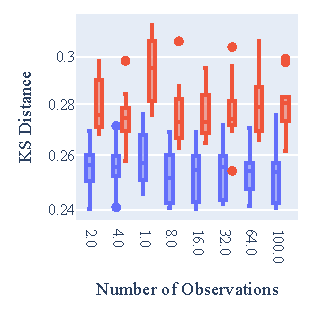
\includegraphics[]{figures/09/figures/performances/clasp_factoring_lognorm_val_ks_d_vs_obs.pdf}
        \caption{Clasp-Factoring}
        \label{fig:ch09:clasp_factoring_ks_d_vs_obs}
    \end{subfigure}
    \begin{subfigure}{0.3\linewidth}
        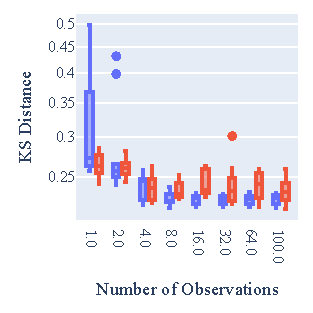
\includegraphics[]{figures/09/figures/performances/saps-CVVAR_lognorm_val_ks_d_vs_obs.pdf}
        \caption{Saps-CV-VAR}
        \label{fig:ch09:saps_cvvar_ks_d_vs_obs}
    \end{subfigure}
    \begin{subfigure}{0.3\linewidth}
        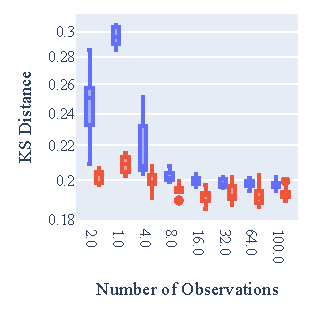
\includegraphics[]{figures/09/figures/performances/spear_qcp_lognorm_val_ks_d_vs_obs.pdf}
        \caption{Spear-QCP}
        \label{fig:ch09:spear_qcp_ks_d_vs_obs}
    \end{subfigure}
    \begin{subfigure}{0.3\linewidth}
        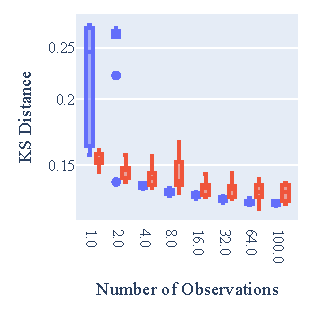
\includegraphics[]{figures/09/figures/performances/yalsat_qcp_lognorm_val_ks_d_vs_obs.pdf}
        \caption{YalSAT-QCP}
        \label{fig:ch09:yalsat_qcp_ks_d_vs_obs}
    \end{subfigure}
    \begin{subfigure}{0.3\linewidth}
        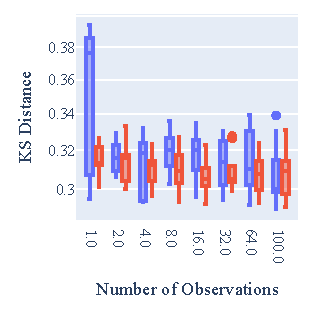
\includegraphics[]{figures/09/figures/performances/spear_swgcp_lognorm_val_ks_d_vs_obs.pdf}
        \caption{Spear-SWGCP}
        \label{fig:ch09:spear_swgcp_ks_d_vs_obs}
    \end{subfigure}
    \begin{subfigure}{0.3\linewidth}
        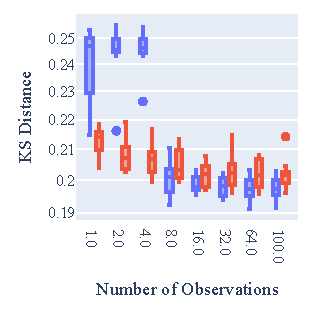
\includegraphics[]{figures/09/figures/performances/yalsat_swgcp_lognorm_val_ks_d_vs_obs.pdf}
        \caption{YalSAT-SWGCP}
        \label{fig:ch09:yalsat_swgcp_ks_d_vs_obs}
    \end{subfigure}
    \begin{subfigure}{0.3\linewidth}
        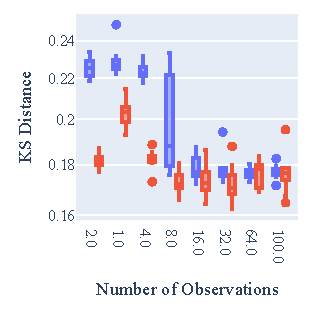
\includegraphics[]{figures/09/figures/performances/lpg-zeno_lognorm_val_ks_d_vs_obs.pdf}
        \caption{LPG-Zenotravel}
        \label{fig:ch09:lpg_zeno_ks_d_vs_obs}
    \end{subfigure}
    \begin{subfigure}{0.3\linewidth}
        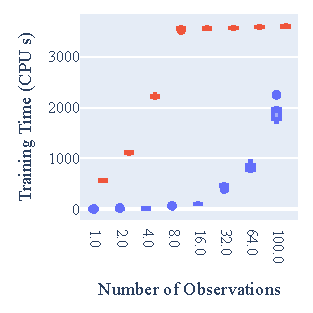
\includegraphics[]{figures/09/figures/performances/saps-CVVAR_lognorm_cpu_training_time_vs_obs.pdf}
        \caption{Saps-CV-VAR (time)}
        \label{fig:ch09:saps_cvvar_cpu_training_time_vs_obs}
    \end{subfigure}
    \begin{subfigure}{0.3\linewidth}
        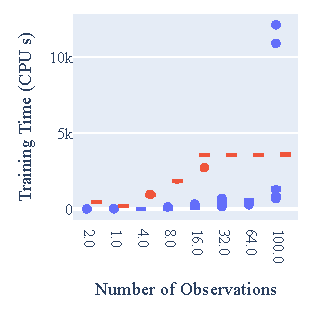
\includegraphics[]{figures/09/figures/performances/lpg-zeno_lognorm_cpu_training_time_vs_obs.pdf}
        \caption{LPG-Zenotravel (time)}
        \label{fig:ch09:lpg_zeno_cpu_training_time_vs_obs}
    \end{subfigure}
    
    \begin{subfigure}{1.0\linewidth}
    \centering
        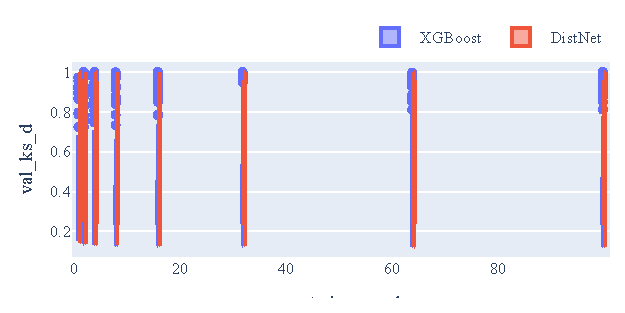
\includegraphics[trim={6.2cm 4.3cm 0cm 0.0cm},clip]{figures/09/figures/performances/legend.pdf}

    \end{subfigure}
    \caption[XGBoost vs DistNet prediction quality]{Prediction quality and training efficiency of XGBoost \emph{vs} DistNet. (a--g) KS distance between predicted and observed running time distributions as a function of the number of training observations per instance, across seven scenarios, predicting the parameters of a \emph{log-normal} distribution; lower is better. XGBoost (blue) performs on par with DistNet (red) across all scenarios, with notable exceptions in the low-data regime, where DistNet retains a performance edge. Both methods improve with more observations added. (h--i) CPU training time comparison on one \gls{sat} and one automated planning scenario. XGBoost requires orders of magnitude less 

    computation (running time) than DistNet while achieving competitive prediction quality. 

    }
    \label{fig:ch09:genperf}
\end{figure}
\FloatBarrier


\subsection{Explainability analysis in SAT: Spear-SWGCP}






We analyse the running time distribution of the Spear \gls{sat} solver on the Small World Graph Colouring Problem (SWGCP)~\citep{GenEtAl99} instances using SATZilla features~\citep{HutEtAl14,ShaHoo24}.
\cref{fig:ch09:spear_swgcp_permut,fig:ch09:spear_swgcp_ice} show permutation importance rankings per statistic and \gls{ice} curves for the top feature per statistic, respectively.
The results reveal a clear structure: the most influential features for the scale statistics (mean, variance and IQR) are local-search probing features, while \gls{dpll} probing features are the most influential for the shape statistics (skewness and kurtosis).

\begin{figure}[!tbp]
    \centering

    \begin{subfigure}{0.3\linewidth}
        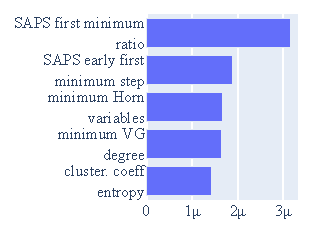
\includegraphics{figures/09/figures/explainability/spear_swgcp_xgb_dist_lognorm_100_fold0_mean_permutation_importance.pdf}
        \caption{Mean}
        \label{fig:ch09:spear_swgcp_mean_permutation_importance}
    \end{subfigure}
    \begin{subfigure}{0.3\linewidth}
        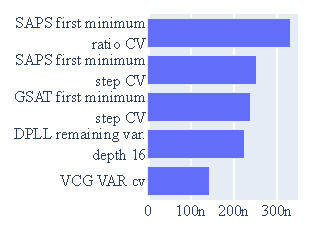
\includegraphics{figures/09/figures/explainability/spear_swgcp_xgb_dist_lognorm_100_fold0_variance_permutation_importance.pdf}
        \caption{Variance}
        \label{fig:ch09:spear_swgcp_variance_permutation_importance}
    \end{subfigure}
    \begin{subfigure}{0.3\linewidth}
        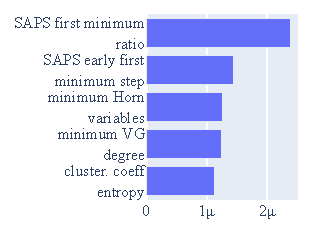
\includegraphics{figures/09/figures/explainability/spear_swgcp_xgb_dist_lognorm_100_fold0_iqr_permutation_importance.pdf}
        \caption{IQR}
        \label{fig:ch09:spear_swgcp_iqr_permutation_importance}
    \end{subfigure}
    \begin{subfigure}{0.3\linewidth}
        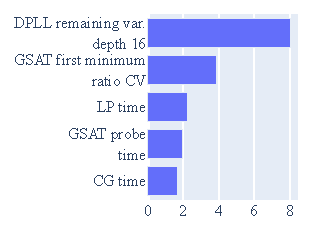
\includegraphics{figures/09/figures/explainability/spear_swgcp_xgb_dist_lognorm_100_fold0_skewness_permutation_importance.pdf}
        \caption{Skewness}
        \label{fig:ch09:spear_swgcp_skewness_permutation_importance}
    \end{subfigure}
    \begin{subfigure}{0.3\linewidth}
        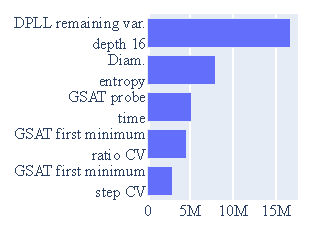
\includegraphics{figures/09/figures/explainability/spear_swgcp_xgb_dist_lognorm_100_fold0_kurtosis_permutation_importance.pdf}
        \caption{Kurtosis}
        \label{fig:ch09:spear_swgcp_kurtosis_permutation_importance}
    \end{subfigure}
    \caption[Permutation importance for Spear on SWGCP]{Permutation importance rankings for the predicted running time distribution statistics of Spear on SWGCP. Mean and IQR are dominated by \gls{saps} local-search probing features, variance by the variability of the same probing signal, and skewness and kurtosis by the number of variables remaining after depth-16 unit-propagation probing.}
    \label{fig:ch09:spear_swgcp_permut}
\end{figure}

For mean and IQR, the most influential feature is the mean ratio of the first local minimum value to the starting value during a short \gls{saps}~\citep{HutEtAl02} local-search run.
\Gls{saps} aims to minimise the number of unsatisfied clauses; therefore, a ratio near 1 means that the first local minimum has an objective value close to the initial one, while a lower value would indicate stronger early improvement.
The \gls{ice} curves show a small step increase in predicted mean and IQR as the ratio moves from approximately 1.0 to 1.06, and the effect is essentially flat for larger values, including the region above 1.1.
This suggests that once early \gls{saps} probing fails to improve beyond the starting objective, the predicted running time and IQR of Spear move to a higher but stable regime.
For prediction of variance, the coefficient of variation of the first local minimum ratio is the most influential feature, with higher variability in local search behaviour across different runs translating to higher variance of the overall running time distribution.
This effect appears early in the observed feature range and then plateaus, suggesting that even moderate instability in the probing signal is enough to identify instances with more variable Spear running times.

Skewness and kurtosis are instead most influenced by the fraction of variables remaining after unit propagation at depth 16 in \gls{dpll} probing, capturing residual formula complexity after simplification rather than local search dynamics.
The corresponding \gls{ice} curves exhibit stronger instance-level heterogeneity than the mean, variance and IQR \gls{saps} features.
Skewness is highest for intermediate fractions of remaining variables, whereas kurtosis decreases substantially as more variables remain after probing.


\begin{figure}[!tbp]
    \centering

    \begin{subfigure}{0.3\linewidth}
        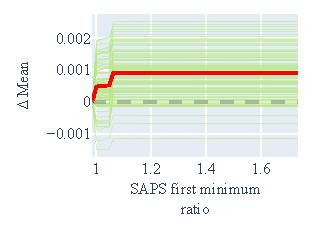
\includegraphics{figures/09/figures/explainability/spear_swgcp_xgb_dist_lognorm_100_fold0_mean_ice_feature59.pdf}
        \caption{Mean }
        \label{fig:ch09:spear_swgcp_mean_ice}
    \end{subfigure}
    \begin{subfigure}{0.3\linewidth}
        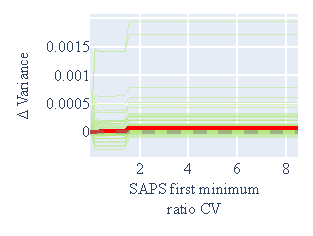
\includegraphics{figures/09/figures/explainability/spear_swgcp_xgb_dist_lognorm_100_fold0_variance_ice_feature60.pdf}
        \caption{\footnotesize Variance}
        \label{fig:ch09:spear_swgcp_variance_ice}
    \end{subfigure}
    \begin{subfigure}{0.3\linewidth}
        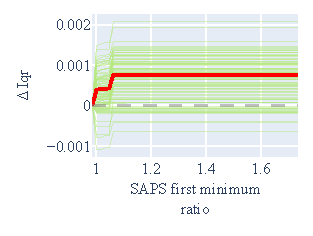
\includegraphics{figures/09/figures/explainability/spear_swgcp_xgb_dist_lognorm_100_fold0_iqr_ice_feature59.pdf}
        \caption{\footnotesize IQR}
        \label{fig:ch09:spear_swgcp_iqr_ice}
    \end{subfigure}
    \begin{subfigure}{0.3\linewidth}
        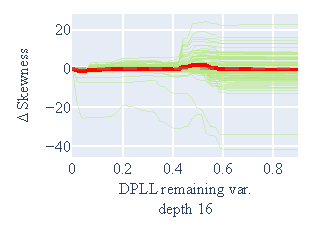
\includegraphics{figures/09/figures/explainability/spear_swgcp_xgb_dist_lognorm_100_fold0_skewness_ice_feature46.pdf}
        \caption{\footnotesize Skewness}
        \label{fig:ch09:spear_swgcp_skewness_ice}
    \end{subfigure}
    \begin{subfigure}{0.3\linewidth}
        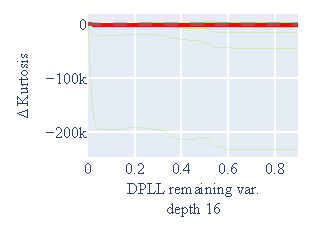
\includegraphics{figures/09/figures/explainability/spear_swgcp_xgb_dist_lognorm_100_fold0_kurtosis_ice_feature46.pdf}
        \caption{Kurtosis}
        \label{fig:ch09:spear_swgcp_kurtosis_ice}
    \end{subfigure}
    \caption[ICE curves for Spear on SWGCP]{Centred \gls{ice} curves for the most important feature of each predicted statistic for Spear on SWGCP. Green curves show individual instances and red curves show partial dependence. The scale statistics change mostly through \gls{saps} first-local-minimum features, while the shape statistics are more heterogeneous and depend on the residual formula size after unit propagation.}
    \label{fig:ch09:spear_swgcp_ice}
\end{figure}
\FloatBarrier
























\subsection{Explainability analysis in automated planning: LPG-Zenotravel}

We analyse the running time distribution of the LPG stochastic local search planner~\citep{GerSer02} on the Zenotravel~\citep{PenWel94} instances.
\cref{fig:ch09:lpg_zeno_permut,fig:ch09:lpg_zeno_ice} show permutation importance rankings per statistic and \gls{ice} curves for the top feature per statistic, respectively.
The planning feature set combines planning-native descriptors, such as \gls{pddl}, causal-graph, domain-transition-graph and probing features, with \gls{sat} features obtained by translating the planning task into a bounded-horizon \gls{cnf} representation~\citep{FawEtAl14}.
In this scenario, the scale statistics (mean, variance, IQR) are driven mainly by features of this \gls{sat} encoding, whereas the shape statistics (skewness, kurtosis) are driven by a planning-native domain-transition-graph feature.

\begin{figure}[!tbp]
    \centering

    \begin{subfigure}{0.3\linewidth}
        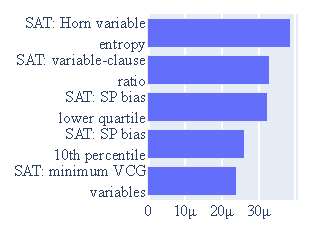
\includegraphics{figures/09/figures/explainability/lpg-zeno_xgb_dist_lognorm_100_fold0_mean_permutation_importance.pdf}
        \caption{Mean}
        \label{fig:ch09:lpg_zeno_mean_permutation_importance}
    \end{subfigure}
    \begin{subfigure}{0.3\linewidth}
        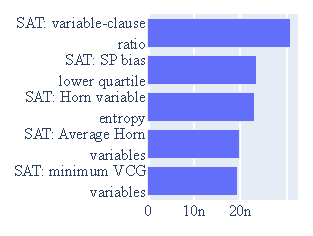
\includegraphics{figures/09/figures/explainability/lpg-zeno_xgb_dist_lognorm_100_fold0_variance_permutation_importance.pdf}
        \caption{Variance}
        \label{fig:ch09:lpg_zeno_variance_permutation_importance}
    \end{subfigure}
    \begin{subfigure}{0.3\linewidth}
        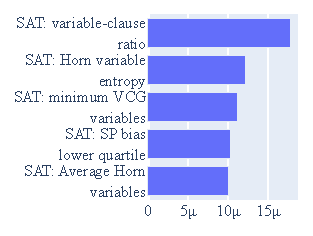
\includegraphics{figures/09/figures/explainability/lpg-zeno_xgb_dist_lognorm_100_fold0_iqr_permutation_importance.pdf}
        \caption{IQR}
        \label{fig:ch09:lpg_zeno_iqr_permutation_importance}
    \end{subfigure}
    \begin{subfigure}{0.3\linewidth}
        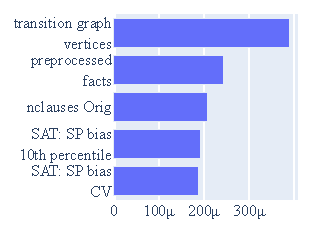
\includegraphics{figures/09/figures/explainability/lpg-zeno_xgb_dist_lognorm_100_fold0_skewness_permutation_importance.pdf}
        \caption{Skewness}
        \label{fig:ch09:lpg_zeno_skewness_permutation_importance}
    \end{subfigure}
    \begin{subfigure}{0.3\linewidth}
        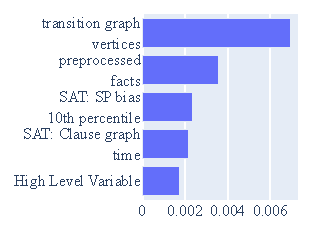
\includegraphics{figures/09/figures/explainability/lpg-zeno_xgb_dist_lognorm_100_fold0_kurtosis_permutation_importance.pdf}
        \caption{Kurtosis}
        \label{fig:ch09:lpg_zeno_kurtosis_permutation_importance}
    \end{subfigure}

    \caption[Permutation importance for LPG on Zenotravel]{Permutation importance rankings for the predicted running time distribution statistics of LPG on Zenotravel. The scale statistics are mainly driven by \gls{sat}-encoding features extracted from the planning task, while skewness and kurtosis are dominated by the size of the planning domain-transition graph.}
    \label{fig:ch09:lpg_zeno_permut}
\end{figure}

For predictions of mean running time, the most influential feature is the entropy of the distribution of Horn-clause variable occurrences in the \gls{sat} encoding.
The proximity-to-Horn features summarise how close the encoded formula is to Horn structure by measuring, for each variable, its occurrence in Horn clauses.
High entropy indicates that this Horn-related structure is spread more uniformly across variables in the bounded planning encoding.
The corresponding \gls{ice} curve shows only a small average effect, but predicted mean running time increases toward the high end of the observed entropy range.
Other highly ranked mean features include the \gls{sat} variable-to-clause ratio and survey-propagation bias features, indicating that central tendency is explained mostly by the constraint structure of the \gls{sat} representation rather than by a single \gls{pddl}-size feature.

For variance and IQR, the top feature is the variable-to-clause ratio of the \gls{sat} encoding.
This ratio is a simple structural measure of the encoded \gls{cnf}: over the observed Zenotravel instances, larger values correspond to fewer clauses per variable and hence lower clause density.
The \gls{ice} curves for variance and IQR are monotonic over the observed range, with both predicted statistics increasing as the variable-to-clause ratio grows.
Thus, the spread of LPG runtimes is associated with how the planning instance is represented as a propositional constraint problem.

Skewness and kurtosis exhibit a different behaviour.
Both skewness and kurtosis are primarily influenced by the total number of vertices in the domain transition graphs, a planning-native feature.
Domain transition graphs describe the possible value transitions of finite-domain planning variables. Their total number of vertices reflects the aggregate size of these variable domains.
The \gls{ice} curves show increasing skewness and kurtosis as this transition structure grows, with the strongest increase near the upper end of the observed range.
This suggests that tail behaviour for LPG-Zenotravel is tied to the size of the underlying finite-domain transition structure, while mean and dispersion are tied more strongly to the bounded \gls{sat} encoding used by the feature extractor.


\begin{figure}[!tbp]
    \centering

    \begin{subfigure}{0.3\linewidth}
        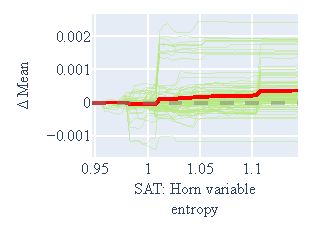
\includegraphics{figures/09/figures/explainability/lpg-zeno_xgb_dist_lognorm_100_fold0_mean_ice_feature2.pdf}
        \caption{Mean}
        \label{fig:ch09:lpg_zeno_mean_ice}
    \end{subfigure}
    \begin{subfigure}{0.3\linewidth}
        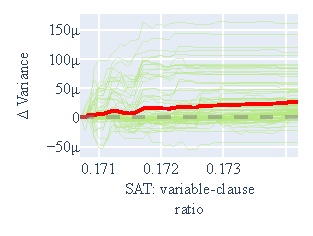
\includegraphics{figures/09/figures/explainability/lpg-zeno_xgb_dist_lognorm_100_fold0_variance_ice_feature62.pdf}
        \caption{Variance}
        \label{fig:ch09:lpg_zeno_variance_ice}
    \end{subfigure}
    \begin{subfigure}{0.3\linewidth}
        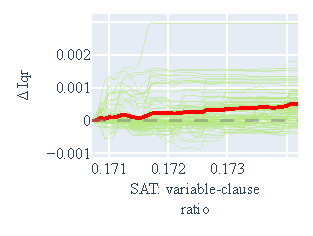
\includegraphics{figures/09/figures/explainability/lpg-zeno_xgb_dist_lognorm_100_fold0_iqr_ice_feature62.pdf}
        \caption{IQR }
        \label{fig:ch09:lpg_zeno_iqr_ice}
    \end{subfigure}
    \begin{subfigure}{0.3\linewidth}
        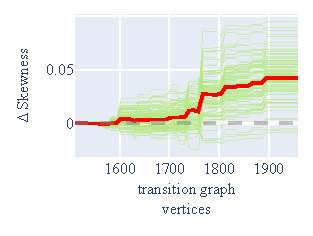
\includegraphics{figures/09/figures/explainability/lpg-zeno_xgb_dist_lognorm_100_fold0_skewness_ice_feature135.pdf}
        \caption{Skewness}
        \label{fig:ch09:lpg_zeno_skewness_ice}
    \end{subfigure}
    \begin{subfigure}{0.3\linewidth}
        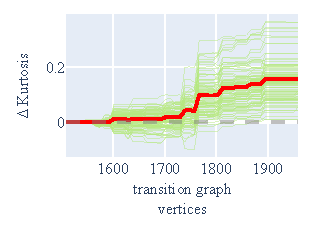
\includegraphics{figures/09/figures/explainability/lpg-zeno_xgb_dist_lognorm_100_fold0_kurtosis_ice_feature135.pdf}
        \caption{Kurtosis}
        \label{fig:ch09:lpg_zeno_kurtosis_ice}
    \end{subfigure}


    \caption[ICE curves for LPG on Zenotravel]{Centred \gls{ice} curves for the most important feature of each predicted statistic for LPG on Zenotravel. Green curves show individual instances and red curves show partial dependence. Horn-variable entropy in the \gls{sat} encoding affect mean running time, the \gls{sat} variable-to-clause ratio governs variance and IQR, and the number of domain-transition-graph vertices affect skewness and kurtosis.}
    \label{fig:ch09:lpg_zeno_ice}
\end{figure}
\FloatBarrier




\section{Chapter conclusion}
\label{sec:ch09:concl}

This chapter proposed a methodology for explaining distribution predictions in the context of algorithm running time distributions.
To this end, it used a probabilistic XGBoost model, which offers a computationally efficient and stable alternative to neural network approaches.
The explanation framework decomposes predicted distributions into interpretable scale and shape statistics, allowing the application of permutation importance and \gls{ice} curves to analyse how specific features influence different aspects of solver performance.

The empirical analysis on \gls{sat} solving and automated planning yields concrete insights for researchers. Specifically, it demonstrated that:
In \gls{sat} solving (specifically, the Spear solver on SWGCP instances), scale statistics (mean and variance) are influenced by early local-search probing dynamics, while shape statistics (skewness and kurtosis) are affected more by \gls{dpll}-simplification features. 
In automated planning (LPG planner on Zenotravel instances), scale statistics are explained by \gls{sat}-encoding characteristics, whereas tail risks are impacted by planning-native domain transition graph sizes. 

This work can be extended in several directions. Firstly, performance distribution prediction has been applied only to running time data of solvers for $\mathcal{NP}$-complete problems. In the future, it is possible to study the performance distributions of additional algorithms for fundamentally different problems, such as machine learning (\emph{e.g.}, training time or hyperparameter tuning stability of deep neural networks). Additionally, while XGBoost matched the predictive quality of DistNet, there remains a gap in modelling low-data regimes (1–8 observations per instance), where neural network approaches still hold a performance edge. Future research can focus on bridging this gap by exploring tree-based architectures with probabilistic priors or hybrid neural-tree models that maintain high explainability without compromising data efficiency.

Overall, the performance of randomised algorithms should not be evaluated and explained based on single statistics, such as the mean, but on the full distribution, to better understand the full range of algorithm behaviour.}

\paragraph{Connection to the thesis}~
This chapter turns empirical performance prediction into a source of scientific insight by explaining not only expected performance, but also variability and tail behaviour.
It shows that prediction models become more useful when their outputs are decomposed into interpretable quantities.
The final technical chapter complements this interpretability perspective with reusable software infrastructure for applying algorithm selection methods across domains.
